\documentclass{standalone}
\usepackage{tikz}
\usetikzlibrary{patterns, positioning}
\usepackage[sfdefault]{ClearSans} %% option 'sfdefault' activates Clear Sans as the default text font
\usepackage[T1]{fontenc}

\begin{document}
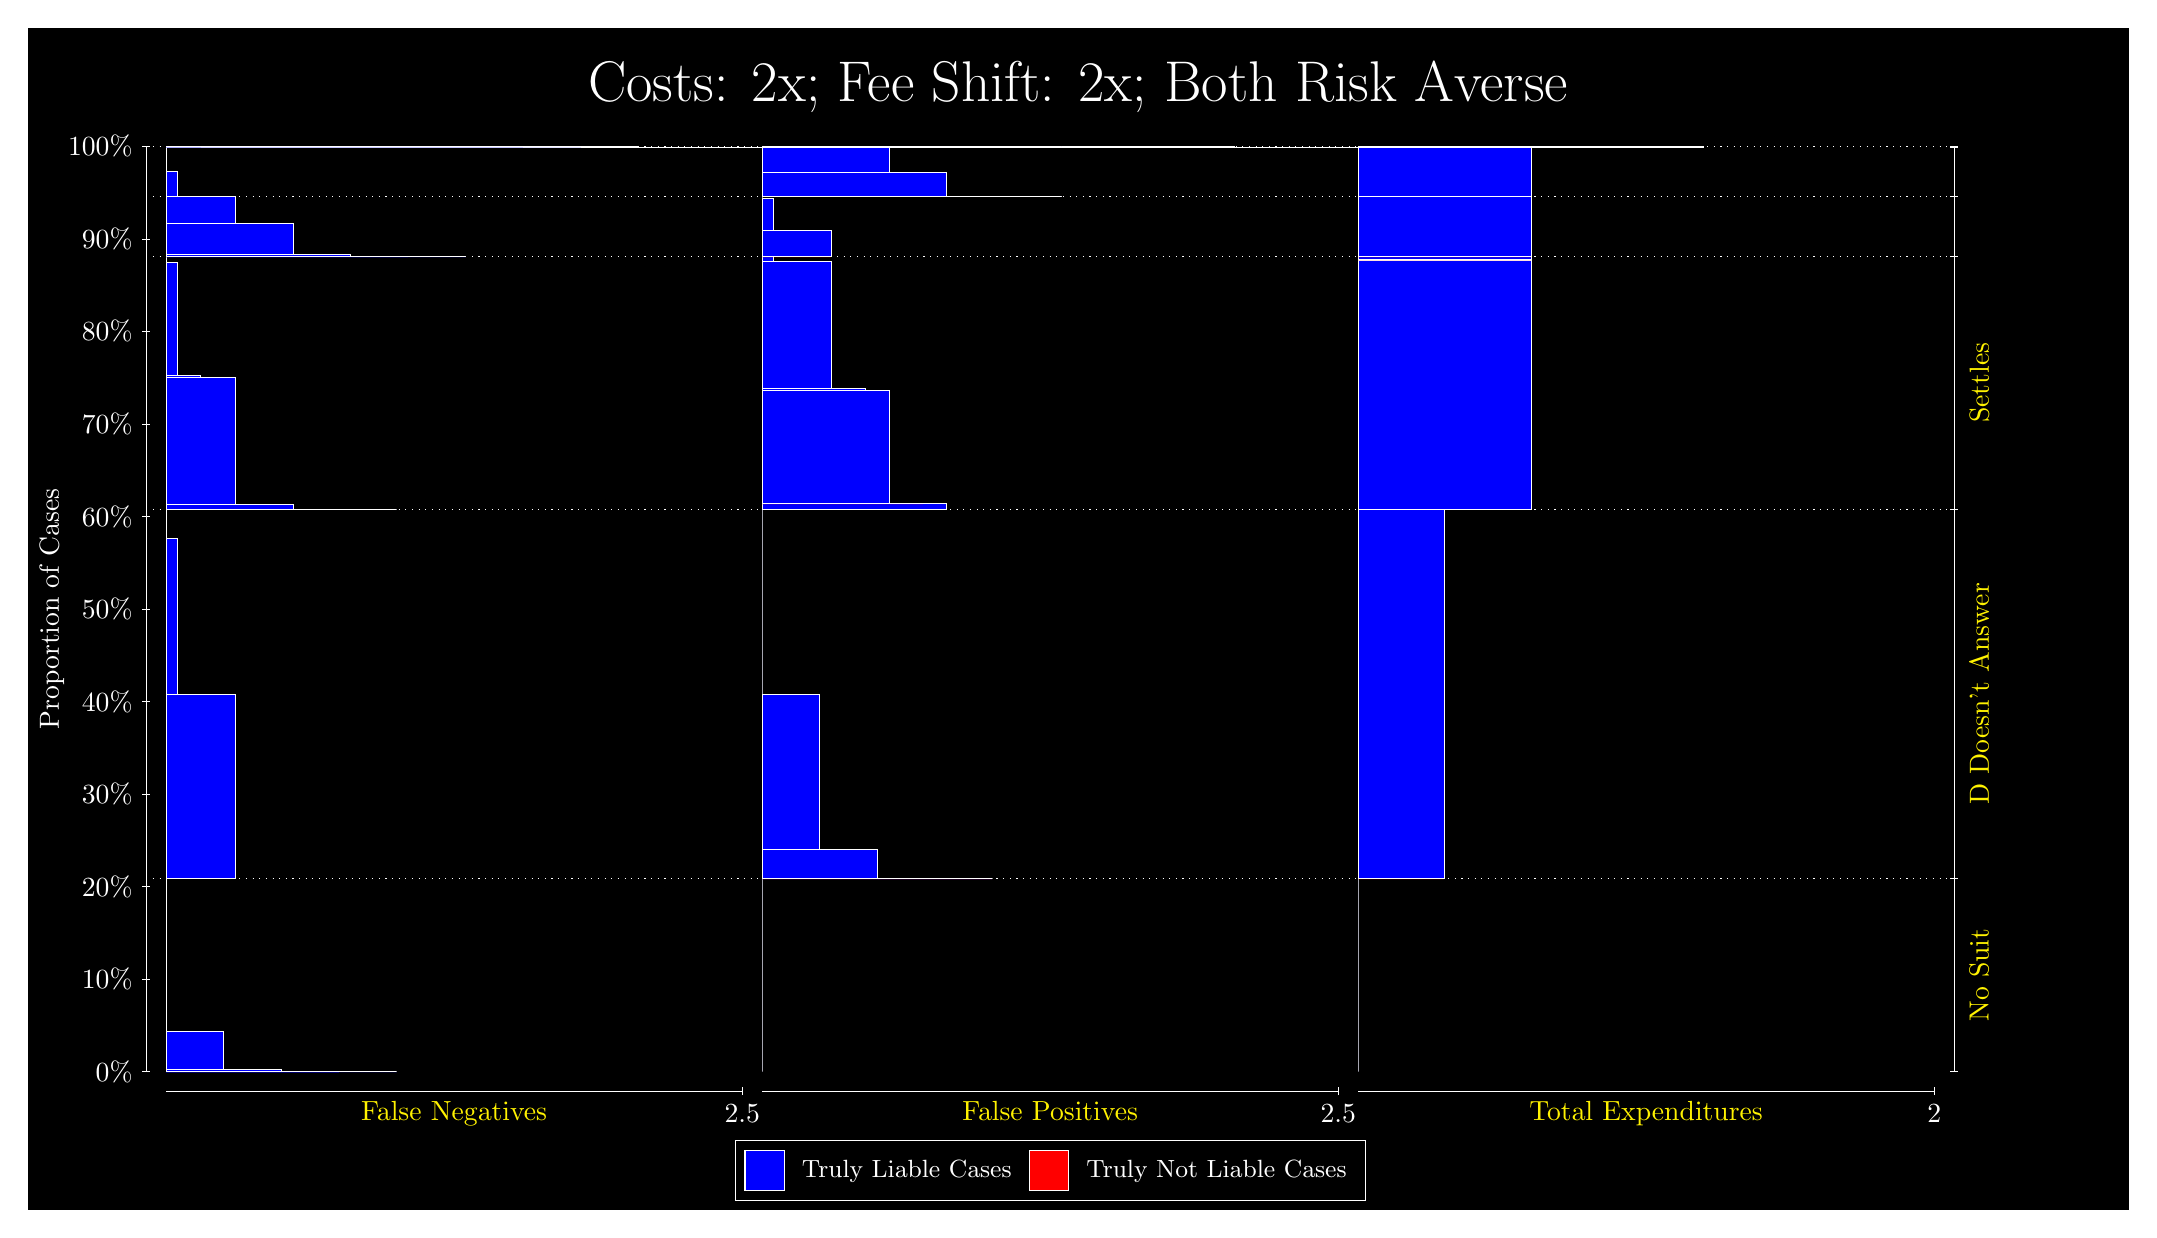
\begin{tikzpicture}
\draw[fill=black] (0,0) rectangle (26.667,15);
\draw[text=white] (0,13.5) rectangle (26.667,15) node[midway] {\huge Costs: 2x; Fee Shift: 2x; Both Risk Averse};
\draw[white, very thin] (1.5,1.75) -- (1.5,13.5);
\node[rotate=90, text=white, anchor=center] at (0.3, 7.625) {Proportion of Cases};
\draw[white, very thin] (1.45,1.75) -- (1.55,1.75);
\node[text=white, anchor=east] at (1.45, 1.75) {0\%};
\draw[white, very thin] (1.45,2.925) -- (1.55,2.925);
\node[text=white, anchor=east] at (1.45, 2.925) {10\%};
\draw[white, very thin] (1.45,4.1) -- (1.55,4.1);
\node[text=white, anchor=east] at (1.45, 4.1) {20\%};
\draw[white, very thin] (1.45,5.275) -- (1.55,5.275);
\node[text=white, anchor=east] at (1.45, 5.275) {30\%};
\draw[white, very thin] (1.45,6.45) -- (1.55,6.45);
\node[text=white, anchor=east] at (1.45, 6.45) {40\%};
\draw[white, very thin] (1.45,7.625) -- (1.55,7.625);
\node[text=white, anchor=east] at (1.45, 7.625) {50\%};
\draw[white, very thin] (1.45,8.8) -- (1.55,8.8);
\node[text=white, anchor=east] at (1.45, 8.8) {60\%};
\draw[white, very thin] (1.45,9.975) -- (1.55,9.975);
\node[text=white, anchor=east] at (1.45, 9.975) {70\%};
\draw[white, very thin] (1.45,11.15) -- (1.55,11.15);
\node[text=white, anchor=east] at (1.45, 11.15) {80\%};
\draw[white, very thin] (1.45,12.325) -- (1.55,12.325);
\node[text=white, anchor=east] at (1.45, 12.325) {90\%};
\draw[white, very thin] (1.45,13.5) -- (1.55,13.5);
\node[text=white, anchor=east] at (1.45, 13.5) {100\%};

\draw[white, very thin] (24.457,1.75) -- (24.457,13.5);
\draw[white, very thin] (24.407,1.75) -- (24.507,1.75);
\node[anchor=west] at (24.407, 1.75) {};
\draw[white, very thin] (24.407,4.1994) -- (24.507,4.1994);
\node[anchor=west] at (24.407, 4.1994) {};
\draw[white, very thin] (24.407,8.8928) -- (24.507,8.8928);
\node[anchor=west] at (24.407, 8.8928) {};
\draw[white, very thin] (24.407,12.1) -- (24.507,12.1);
\node[anchor=west] at (24.407, 12.1) {};
\draw[white, very thin] (24.407,12.865) -- (24.507,12.865);
\node[anchor=west] at (24.407, 12.865) {};
\draw[white, very thin] (24.407,13.494) -- (24.507,13.494);
\node[anchor=west] at (24.407, 13.494) {};
\draw[white, very thin] (24.407,13.5) -- (24.507,13.5);
\node[anchor=west] at (24.407, 13.5) {};

\draw[white, very thin, fill=blue] (1.75,1.75) rectangle (4.6775,1.75);
\draw[white, very thin, fill=blue] (1.75,1.75) rectangle (3.9457,1.7502);
\draw[white, very thin, fill=blue] (1.75,1.7502) rectangle (3.2138,1.7793);
\draw[white, very thin, fill=blue] (1.75,1.7793) rectangle (2.4819,2.2618);
\draw[white, very thin, fill=red] (1.75,2.2618) rectangle (1.75,2.2618);
\draw[white, very thin, fill=blue] (1.75,2.2618) rectangle (1.75,4.1994);
\draw[white, very thin, fill=blue] (1.75,4.1994) rectangle (2.6283,6.5456);
\draw[white, very thin, fill=blue] (1.75,6.5456) rectangle (1.8964,8.5221);
\draw[white, very thin, fill=red] (1.75,8.5221) rectangle (1.75,8.5221);
\draw[white, very thin, fill=blue] (1.75,8.5221) rectangle (1.75,8.8928);
\draw[white, very thin, fill=blue] (1.75,8.8928) rectangle (4.6775,8.8928);
\draw[white, very thin, fill=blue] (1.75,8.8928) rectangle (4.3848,8.8928);
\draw[white, very thin, fill=blue] (1.75,8.8928) rectangle (4.092,8.8928);
\draw[white, very thin, fill=blue] (1.75,8.8928) rectangle (3.9457,8.8928);
\draw[white, very thin, fill=blue] (1.75,8.8928) rectangle (3.6529,8.8928);
\draw[white, very thin, fill=blue] (1.75,8.8928) rectangle (3.3602,8.9521);
\draw[white, very thin, fill=blue] (1.75,8.9521) rectangle (3.2138,8.9522);
\draw[white, very thin, fill=blue] (1.75,8.9522) rectangle (2.921,8.9595);
\draw[white, very thin, fill=blue] (1.75,8.9595) rectangle (2.6283,10.563);
\draw[white, very thin, fill=blue] (1.75,10.563) rectangle (2.4819,10.567);
\draw[white, very thin, fill=blue] (1.75,10.567) rectangle (2.1891,10.597);
\draw[white, very thin, fill=blue] (1.75,10.597) rectangle (1.8964,12.026);
\draw[white, very thin, fill=red] (1.75,12.026) rectangle (1.75,12.026);
\draw[white, very thin, fill=blue] (1.75,12.026) rectangle (1.75,12.1);
\draw[white, very thin, fill=blue] (1.75,12.1) rectangle (5.5558,12.1);
\draw[white, very thin, fill=blue] (1.75,12.1) rectangle (4.8239,12.1);
\draw[white, very thin, fill=blue] (1.75,12.1) rectangle (4.092,12.129);
\draw[white, very thin, fill=blue] (1.75,12.129) rectangle (3.3602,12.527);
\draw[white, very thin, fill=blue] (1.75,12.527) rectangle (2.6283,12.865);
\draw[white, very thin, fill=red] (1.75,12.865) rectangle (1.75,12.865);
\draw[white, very thin, fill=blue] (1.75,12.865) rectangle (2.6283,12.869);
\draw[white, very thin, fill=blue] (1.75,12.869) rectangle (1.8964,13.183);
\draw[white, very thin, fill=red] (1.75,13.183) rectangle (1.75,13.183);
\draw[white, very thin, fill=blue] (1.75,13.183) rectangle (1.75,13.494);
\draw[white, very thin, fill=blue] (1.75,13.494) rectangle (9.9471,13.494);
\draw[white, very thin, fill=blue] (1.75,13.494) rectangle (9.2152,13.494);
\draw[white, very thin, fill=blue] (1.75,13.494) rectangle (8.4834,13.494);
\draw[white, very thin, fill=blue] (1.75,13.494) rectangle (7.7515,13.495);
\draw[white, very thin, fill=blue] (1.75,13.495) rectangle (7.0196,13.495);
\draw[white, very thin, fill=blue] (1.75,13.495) rectangle (6.2877,13.495);
\draw[white, very thin, fill=blue] (1.75,13.495) rectangle (2.1891,13.495);
\draw[white, very thin, fill=red] (1.75,13.495) rectangle (1.75,13.495);
\draw[white, very thin, fill=blue] (1.75,13.495) rectangle (1.75,13.5);
\draw[white, very thin, fill=red] (9.3189,1.75) rectangle (9.3189,1.75);
\draw[white, very thin, fill=blue] (9.3189,1.75) rectangle (9.3189,4.1994);
\draw[white, very thin, fill=red] (9.3189,4.1994) rectangle (12.246,4.1994);
\draw[white, very thin, fill=blue] (9.3189,4.1994) rectangle (12.246,4.1994);
\draw[white, very thin, fill=blue] (9.3189,4.1994) rectangle (11.515,4.2019);
\draw[white, very thin, fill=blue] (9.3189,4.2019) rectangle (10.783,4.5702);
\draw[white, very thin, fill=blue] (9.3189,4.5702) rectangle (10.051,6.5467);
\draw[white, very thin, fill=blue] (9.3189,6.5467) rectangle (9.3189,8.8928);
\draw[white, very thin, fill=red] (9.3189,8.8928) rectangle (11.661,8.8928);
\draw[white, very thin, fill=blue] (9.3189,8.8928) rectangle (11.661,8.9622);
\draw[white, very thin, fill=red] (9.3189,8.9622) rectangle (11.368,8.9622);
\draw[white, very thin, fill=blue] (9.3189,8.9622) rectangle (11.368,8.964);
\draw[white, very thin, fill=red] (9.3189,8.964) rectangle (11.075,8.964);
\draw[white, very thin, fill=blue] (9.3189,8.964) rectangle (11.075,8.9669);
\draw[white, very thin, fill=blue] (9.3189,8.9669) rectangle (10.929,10.396);
\draw[white, very thin, fill=blue] (9.3189,10.396) rectangle (10.636,10.426);
\draw[white, very thin, fill=blue] (9.3189,10.426) rectangle (10.344,10.431);
\draw[white, very thin, fill=blue] (9.3189,10.431) rectangle (10.197,12.034);
\draw[white, very thin, fill=blue] (9.3189,12.034) rectangle (9.9044,12.041);
\draw[white, very thin, fill=blue] (9.3189,12.041) rectangle (9.6116,12.041);
\draw[white, very thin, fill=blue] (9.3189,12.041) rectangle (9.4652,12.1);
\draw[white, very thin, fill=blue] (9.3189,12.1) rectangle (9.3189,12.1);
\draw[white, very thin, fill=red] (9.3189,12.1) rectangle (10.197,12.1);
\draw[white, very thin, fill=blue] (9.3189,12.1) rectangle (10.197,12.439);
\draw[white, very thin, fill=blue] (9.3189,12.439) rectangle (9.4652,12.837);
\draw[white, very thin, fill=blue] (9.3189,12.837) rectangle (9.3189,12.865);
\draw[white, very thin, fill=red] (9.3189,12.865) rectangle (13.125,12.865);
\draw[white, very thin, fill=blue] (9.3189,12.865) rectangle (13.125,12.865);
\draw[white, very thin, fill=blue] (9.3189,12.865) rectangle (12.393,12.868);
\draw[white, very thin, fill=blue] (9.3189,12.868) rectangle (11.661,13.176);
\draw[white, very thin, fill=blue] (9.3189,13.176) rectangle (10.929,13.49);
\draw[white, very thin, fill=blue] (9.3189,13.49) rectangle (10.197,13.494);
\draw[white, very thin, fill=red] (9.3189,13.494) rectangle (17.516,13.494);
\draw[white, very thin, fill=blue] (9.3189,13.494) rectangle (17.516,13.494);
\draw[white, very thin, fill=red] (9.3189,13.494) rectangle (16.784,13.494);
\draw[white, very thin, fill=blue] (9.3189,13.494) rectangle (16.784,13.494);
\draw[white, very thin, fill=red] (9.3189,13.494) rectangle (16.052,13.494);
\draw[white, very thin, fill=blue] (9.3189,13.494) rectangle (16.052,13.494);
\draw[white, very thin, fill=red] (9.3189,13.494) rectangle (15.32,13.494);
\draw[white, very thin, fill=blue] (9.3189,13.494) rectangle (15.32,13.495);
\draw[white, very thin, fill=blue] (9.3189,13.495) rectangle (14.588,13.498);
\draw[white, very thin, fill=blue] (9.3189,13.498) rectangle (13.857,13.498);
\draw[white, very thin, fill=blue] (9.3189,13.498) rectangle (13.125,13.498);
\draw[white, very thin, fill=blue] (9.3189,13.498) rectangle (12.393,13.498);
\draw[white, very thin, fill=red] (9.3189,13.498) rectangle (9.3189,13.498);
\draw[white, very thin, fill=blue] (9.3189,13.498) rectangle (9.3189,13.5);
\draw[white, very thin, fill=red] (16.888,1.75) rectangle (16.888,1.75);
\draw[white, very thin, fill=blue] (16.888,1.75) rectangle (16.888,4.1994);
\draw[white, very thin, fill=red] (16.888,4.1994) rectangle (17.986,4.1994);
\draw[white, very thin, fill=blue] (16.888,4.1994) rectangle (17.986,8.8928);
\draw[white, very thin, fill=red] (16.888,8.8928) rectangle (19.083,8.8928);
\draw[white, very thin, fill=blue] (16.888,8.8928) rectangle (19.083,12.054);
\draw[white, very thin, fill=red] (16.888,12.054) rectangle (19.083,12.054);
\draw[white, very thin, fill=blue] (16.888,12.054) rectangle (19.083,12.061);
\draw[white, very thin, fill=red] (16.888,12.061) rectangle (19.083,12.061);
\draw[white, very thin, fill=blue] (16.888,12.061) rectangle (19.083,12.1);
\draw[white, very thin, fill=red] (16.888,12.1) rectangle (19.083,12.1);
\draw[white, very thin, fill=blue] (16.888,12.1) rectangle (19.083,12.865);
\draw[white, very thin, fill=red] (16.888,12.865) rectangle (19.083,12.865);
\draw[white, very thin, fill=blue] (16.888,12.865) rectangle (19.083,13.494);
\draw[white, very thin, fill=red] (16.888,13.494) rectangle (21.279,13.494);
\draw[white, very thin, fill=blue] (16.888,13.494) rectangle (21.279,13.5);
\draw[white, dotted] (1.5,4.1994) -- (24.457,4.1994);
\draw[white, dotted] (1.5,8.8928) -- (24.457,8.8928);
\draw[white, dotted] (1.5,12.1) -- (24.457,12.1);
\draw[white, dotted] (1.5,12.865) -- (24.457,12.865);
\draw[white, dotted] (1.5,13.494) -- (24.457,13.494);
\draw[white, very thin] (1.75,1.5) -- (9.0689,1.5);
\node[text=yellow, anchor=north] at (5.4094, 1.5) {False Negatives};
\draw[white, very thin] (9.0689,1.45) -- (9.0689,1.55);
\node[text=white, anchor=north] at (9.0689, 1.45) {2.5};

\draw[white, very thin] (9.3189,1.5) -- (16.638,1.5);
\node[text=yellow, anchor=north] at (12.978, 1.5) {False Positives};
\draw[white, very thin] (16.638,1.45) -- (16.638,1.55);
\node[text=white, anchor=north] at (16.638, 1.45) {2.5};

\draw[white, very thin] (16.888,1.5) -- (24.207,1.5);
\node[text=yellow, anchor=north] at (20.547, 1.5) {Total Expenditures};
\draw[white, very thin] (24.207,1.45) -- (24.207,1.55);
\node[text=white, anchor=north] at (24.207, 1.45) {2};

\node[text=yellow, centered, rotate=90] at (24.777, 2.9747) {No Suit};
\node[text=yellow, centered, rotate=90] at (24.777, 6.5461) {D Doesn't Answer};
\node[text=yellow, centered, rotate=90] at (24.777, 10.497) {Settles};




\draw (12.978300999999998,1.5) node[draw=none] (baseCoordinate) {};
\begin{scope}[align=center]
        \matrix[scale=0.5, draw=white, below=0.5cm of baseCoordinate, nodes={draw}, column sep=0.1cm]{
            \node[rectangle, draw, minimum width=0.5cm, minimum height=0.5cm, fill=blue] {}; &
            \node[draw=none, font=\small, text=white] (B) {Truly Liable Cases}; &
            \node[rectangle, draw, minimum width=0.5cm, minimum height=0.5cm, fill=red] {}; &
            \node[draw=none, font=\small, text=white] (B) {Truly Not Liable Cases}; \\
            };
\end{scope}

\end{tikzpicture}
\end{document}